\chapter{Effects of Variation on the Evolution of Larval Trait Parameters}
Stochasticity in the model comes from initial standing variation in larval trait parameters as well as from heritability of each trait parameter during the inheritance of those traits. The results from simulations show how these sources of variations play an important role in determining the evolutionary routes taken to increase fitness and achieve greater competitive ability.
\section{Variation in the Initial Distribution of Larval Trait Parameters}
In the initial distribution of each trait value, the variation comes from the standard deviation given for each distribution of the traits like feeding rate, waste tolerance, critical size and efficiency. The initial standing variation in these trait distributions determines the maximum mean trait value that can be achieved to increase the fitness. Simulations were performed for given fixed mean trait values but varying their respective initial standing variation in MB, MCU and CCU cultures (generations = 50, replicates = 5). These simulations were aimed at investigating how these variations interact in order to obtain maximum fitness. In fig~\ref{fig:ivar_fr_eff} - ~\ref{fig:ivar_mc_eff}, differences of the mean trait values of the population at $50^{th}$ generation and $0^{th}$ generation are plotted for different combinations of initial variation in trait values. The initial standard deviation for a trait is taken as a certain percentage of its respective mean trait value at $0^{th}$ generation given in table~\ref{tab:trait_value}.\\\\
These results show that differences in variation of these trait parameters give different mean trait values at $50^{th}$ generation across different crowding densities. Overall there is no significant effect of initial variation in trait parameters on the mean trait values in MB culture. Higher initial variation in initial feeding rate and efficiency give higher mean initial feeding rate and mean efficiency respectively after $50^{th}$ generation in MCU and CCU cultures without showing any interaction (see fig~\ref{fig:ivar_fr_eff}). There is no difference between the mean trait value of efficiency of MCU and CCU cultures. Mean initial feeding rate evolved in MCU culture is lesser than in CCU culture only when initial variation in this trait is high(see fig~\ref{fig:ivar_fr_mc}). There is no significant effect on the mean critical size at $50^{th}$ generation due to initial variation in initial feeding rate and critical size at all densities. In Fig~\ref{fig:ivar_mc_eff}, initial variation in efficiency and critical size both interact with each other, which gives a significant difference in mean efficiency between MCU and CCU cultures. At lower initial variation of efficiency, there is no effect of initial variation in critical size on the mean efficiency (see fig~\ref{fig:ivar_mc_eff}). This pattern is similar in MCU and CCU cultures. Higher initial variation in the efficiency and higher initial variation in critical size, both together lead to a difference in mean efficiency across MCU and CCU culture. At higher initial variation in efficiency but lower variation in critical size, there is no significant difference in mean efficiency across MCU and CCU culture. Fig~\ref{fig:ivar_mc_eff} shows the interaction of initial variation in efficiency and critical size in achieving higher efficiency across MCU and CCU cultures. There is no effect of these variations on mean critical size. There was no effect of these variations on waste tolerance, and the graphs are given in appendix A2.
\begin{figure}[p]
  \subfloat{
  \centering
  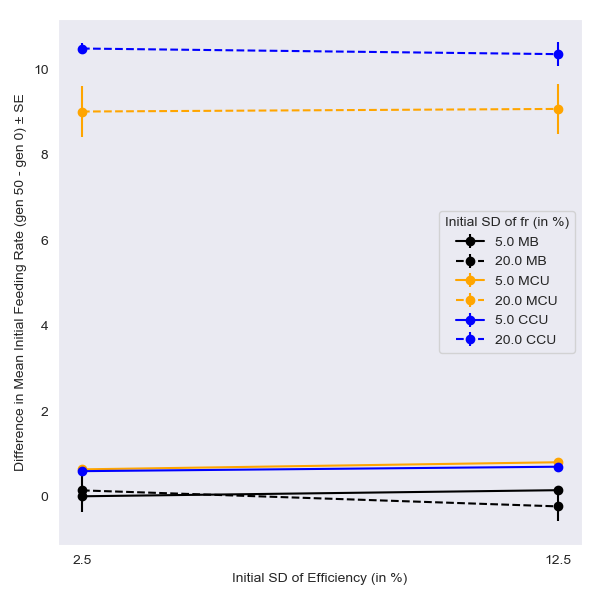
\includegraphics[width=0.5\textwidth]{C5/Figs/ivar/ivar_fr_eff_fr}
  }
  \subfloat{
  \centering
  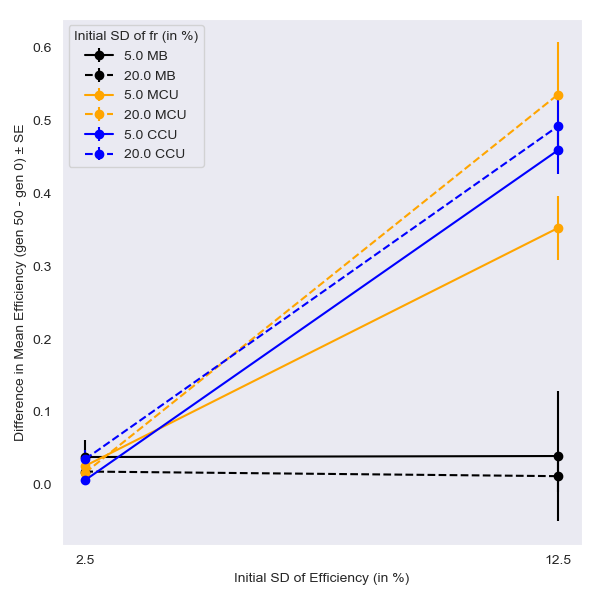
\includegraphics[width=0.5\textwidth]{C5/Figs/ivar/ivar_fr_eff_eff}
  }
  \caption{Effect of initial variation in initial feeding rate and efficiency.}
  \label{fig:ivar_fr_eff}
\end{figure}
\begin{figure}[p]
  \subfloat{
  \centering
  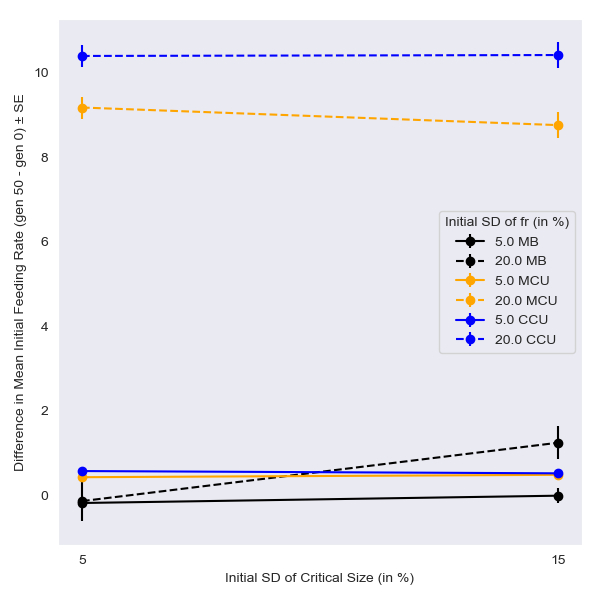
\includegraphics[width=0.5\textwidth]{C5/Figs/ivar/ivar_fr_mc_fr}
  }
  \subfloat{
  \centering
  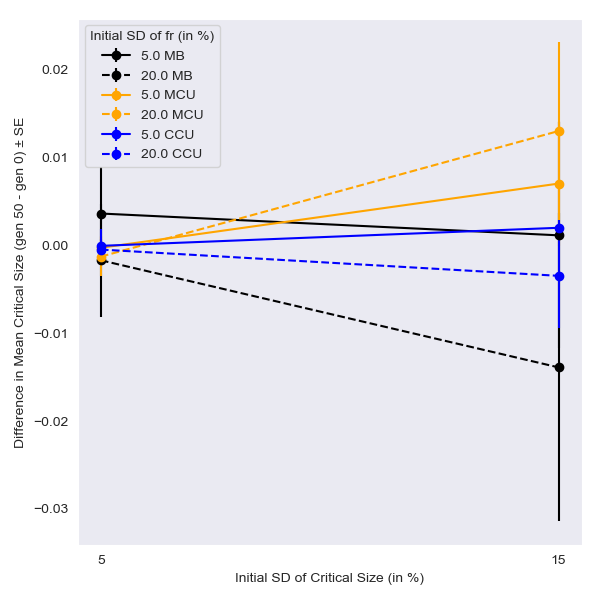
\includegraphics[width=0.5\textwidth]{C5/Figs/ivar/ivar_fr_mc_mc}
  }
  \caption{Effect of initial variation in initial feeding rate and critical size.}
  \label{fig:ivar_fr_mc}
\end{figure}
\clearpage

\begin{figure}[t]
  \subfloat{
  \centering
  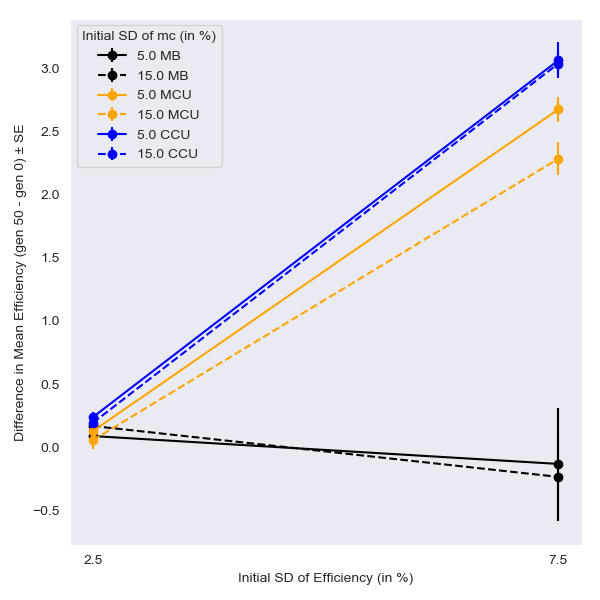
\includegraphics[width=0.5\textwidth]{C5/Figs/ivar/ivar_mc_eff_eff}
  }
  \subfloat{
  \centering
  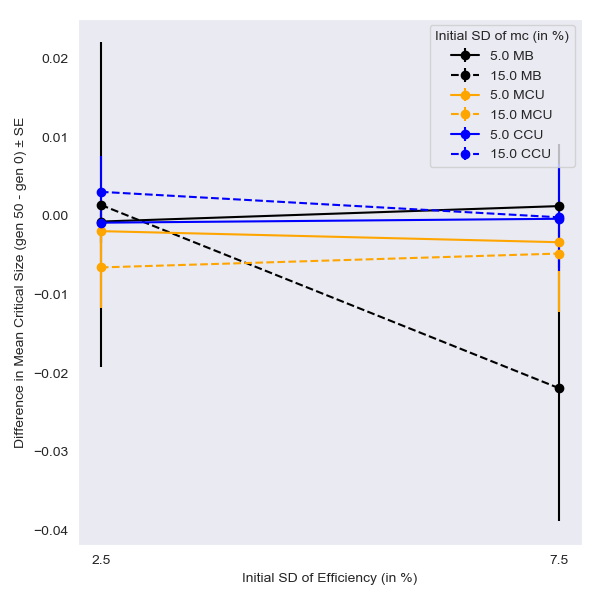
\includegraphics[width=0.5\textwidth]{C5/Figs/ivar/ivar_mc_eff_mc}
  }
  \caption{Effect of initial variation in critical size and efficiency.}
  \label{fig:ivar_mc_eff}
\end{figure}

\section{Heritability of Larval Trait Parameters}
During the inheritance of trait parameters from parents to offspring, the variation in the trait value of offspring from the parents comes from heritability of that trait parameter. In the model, trait values are assigned to offspring from a normal distribution around mid-parent value as mean, and a certain standard deviation ($\omega$). This standard deviation, $\omega$,   in the respective trait distribution is taken as a measure of heritability for that trait. It is taken as a certain percentage of the mean value of the respective trait parameter at $0^{th}$ generation. Higher the standard deviation, lesser is heritability for that trait parameter. For fixed initial conditions, simulations are performed with varying $\omega$ for combinations of trait parameters across MB, MCU and CCU cultures (see table~\ref{tab:trait_value}, generations = 50, replicates = 5). The results from these simulations are plotted similar to initial variation plots (see fig~\ref{fig:omg_fr_eff} - \ref{fig:omg_mc_eff}).\\\\
Results from these simulations show that initial feeding rate, efficiency and critical size do not show any significant effect of heritability of these trait parameters in MB culture. Higher heritability of initial feeding rate leads to higher mean initial feeding rate in both MCU and CCU culture. In MCU and CCU cultures, mean initial feeding rate decreases with a decrease in the heritability of efficiency only for higher heritability of initial feeding rate. Otherwise, such interaction of mean initial feeding rate with the heritability of efficiency is only observed in CCU culture at low heritability of initial feeding rate (fig~\ref{fig:omg_fr_eff}). The only significant difference in mean efficiency is between MCU and CCU culture when heritability of efficiency is less. Mean critical size is not affected by heritability of these two trait parameters at all densities. Lower heritability of efficiency also seems to cause an increase in mean waste tolerance without any interaction in all cultures.
\begin{figure}[h]
  \subfloat{
  \centering
  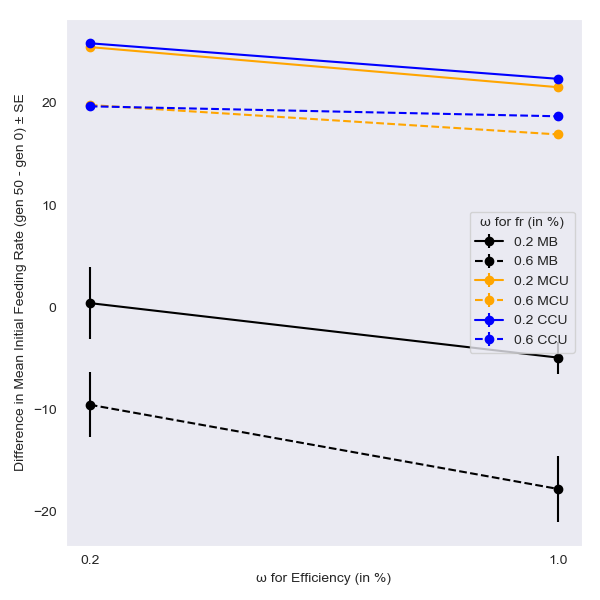
\includegraphics[width=0.5\textwidth]{C5/Figs/omg/omega_fr_eff_fr}
  }
  \subfloat{
  \centering
  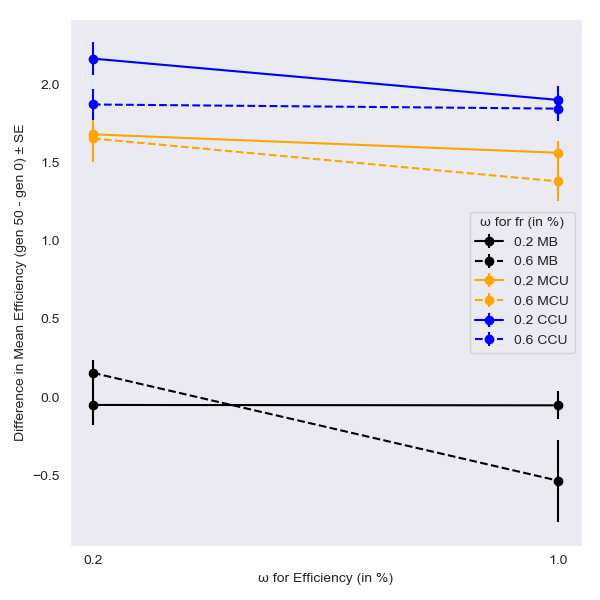
\includegraphics[width=0.5\textwidth]{C5/Figs/omg/omega_fr_eff_eff}
  }\\
  \subfloat{
  \centering
  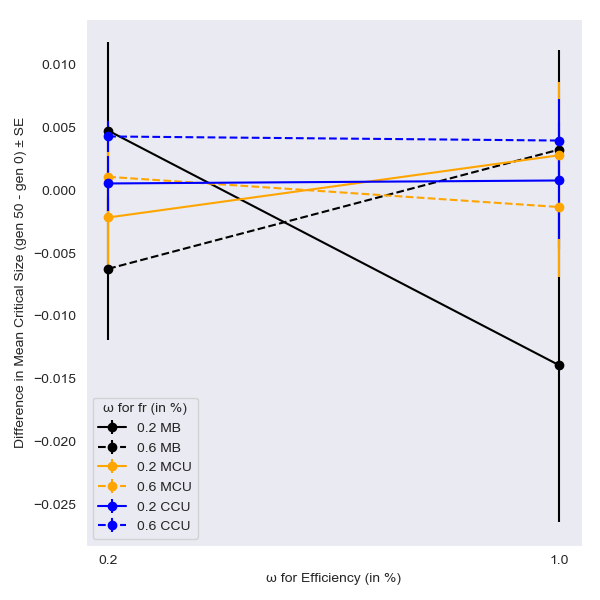
\includegraphics[width=0.5\textwidth]{C5/Figs/omg/omega_fr_eff_mc}
  }
  \subfloat{
  \centering
  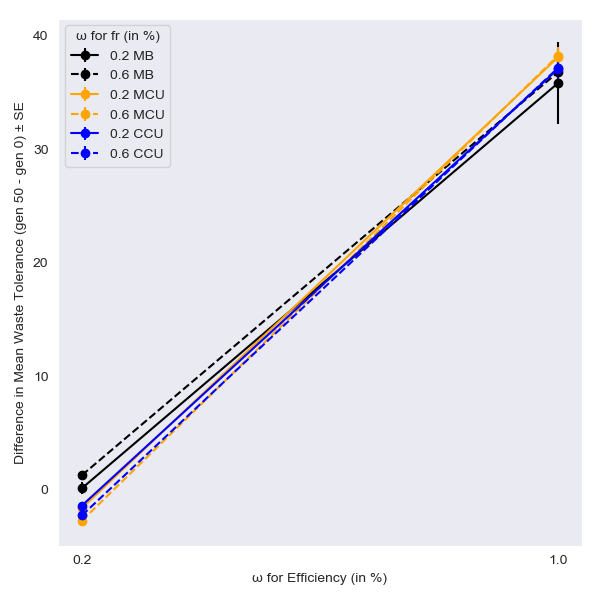
\includegraphics[width=0.5\textwidth]{C5/Figs/omg/omega_fr_eff_wtol}
  }
  \caption{Effect of heritability in initial feeding rate (fr) and efficiency on mean trait values at generation 50.}
  \label{fig:omg_fr_eff}
\end{figure}
\clearpage

\noindent Fig~\ref{fig:omg_fr_mc} shows that a decrease in heritability of critical size decreases mean initial feeding rate in both MCU and CCU cultures only when the heritability of initial feeding rate is high. Such effect is also seen at lower heritability of initial feeding rate only in CCU culture when (fig~\ref{fig:omg_fr_mc}). In MCU culture, mean efficiency increases with an increase in the heritability of initial feeding rate at higher heritability of critical size. In contrast, there is no effect of heritability of initial feeding rate on mean efficiency when heritability of critical size lower in MCU culture. This pattern of mean efficiency with a heritability of these trait parameters is opposite in CCU culture. In MCU and CCU cultures, higher heritability of critical size causes no change in mean critical size over generations. Lower heritability of critical size causes a decrease in mean critical size in MCU and CCU cultures equally. This decrease shows interaction with the heritability of initial feeding rate, as higher heritability of initial feeding rate gives more decrease in mean critical size in both MCU and CCU cultures. There is no effect of the heritability of these trait parameters on mean waste tolerance.\\\\
Fig~\ref{fig:omg_mc_eff} shows overall no significant effect of heritability of critical size on the mean initial feeding rate. At higher heritability of efficiency, the mean initial feeding rate shows the difference between MCU and CCU culture. This difference between MCU and CCU cultures disappears at lower heritability of efficiency. Mean efficiency is higher for lower heritability of efficiency and higher heritability of critical size in MCU and CCU cultures. There is no effect of heritability of critical size on mean efficiency at higher heritability of efficiency in MCU culture. Mean efficiency between MCU and CCU culture is different when heritability of efficiency higher and that of critical size is lower. There is no effect of heritability of efficiency on mean critical size. Heritability of critical size only affects mean critIcal size when heritability of efficiency is high. Mean waste tolerance has a pattern similar to fig~\ref{fig:omg_fr_eff}, showing that it is dependent on the heritability of efficiency.
\begin{figure}[p]
  \subfloat{
  \centering
  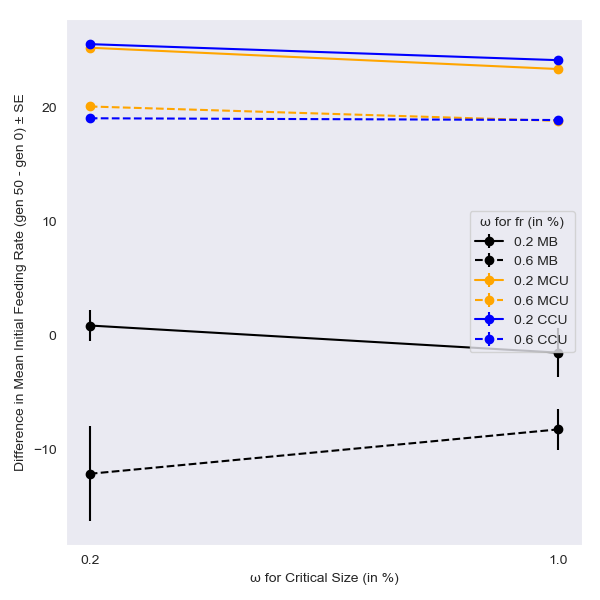
\includegraphics[width=0.5\textwidth]{C5/Figs/omg/omega_fr_mc_fr}
  }
  \subfloat{
  \centering
  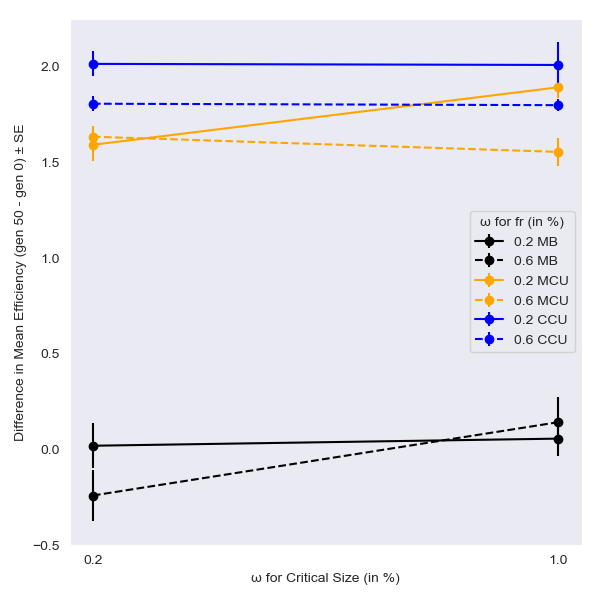
\includegraphics[width=0.5\textwidth]{C5/Figs/omg/omega_fr_mc_eff}
  }\\
  \subfloat{
  \centering
  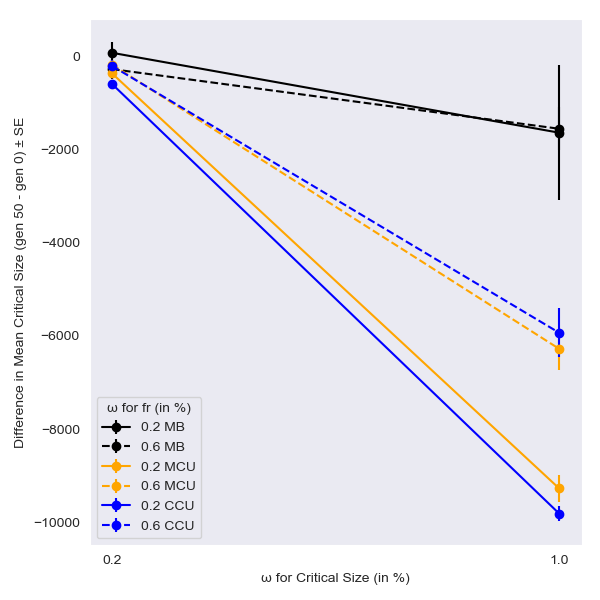
\includegraphics[width=0.5\textwidth]{C5/Figs/omg/omega_fr_mc_mc}
  }
  \subfloat{
  \centering
  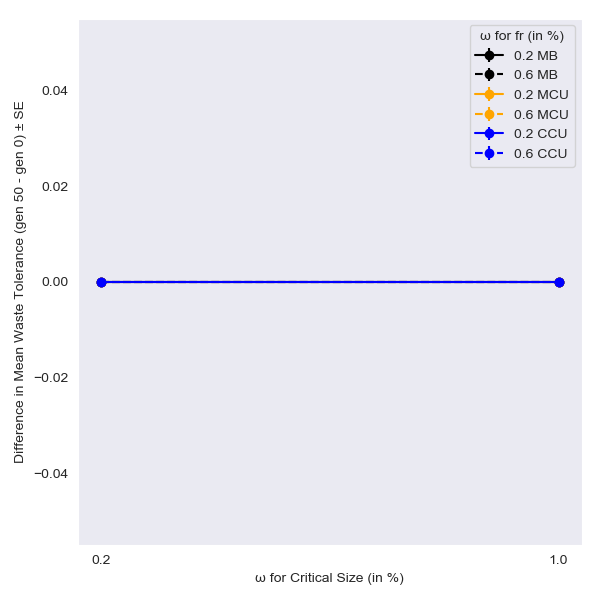
\includegraphics[width=0.5\textwidth]{C5/Figs/omg/omega_fr_mc_wtol}
  }
  \caption{Effect of heritability in initial feeding rate (fr) and critical size on mean trait values at generation 50.}
  \label{fig:omg_fr_mc}
\end{figure}
\begin{figure}[p]
  \subfloat{
  \centering
  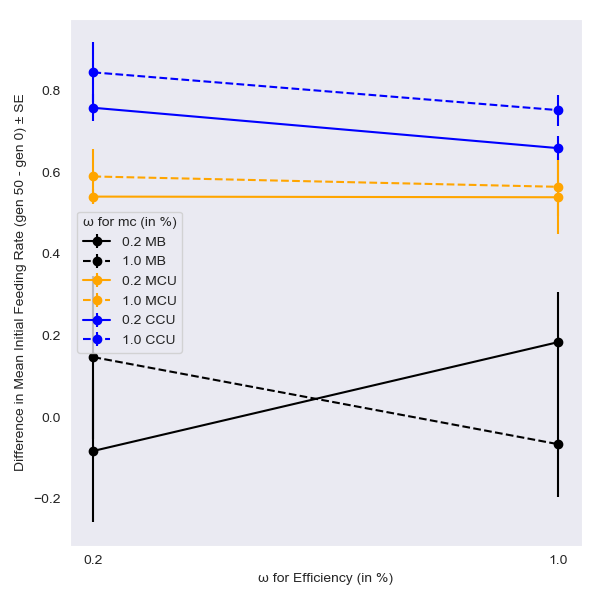
\includegraphics[width=0.5\textwidth]{C5/Figs/omg/omega_mc_eff_fr}
  }
  \subfloat{
  \centering
  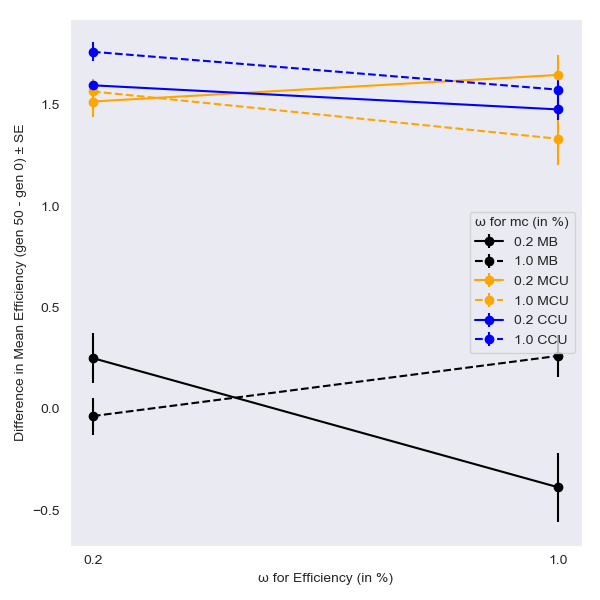
\includegraphics[width=0.5\textwidth]{C5/Figs/omg/omega_mc_eff_eff}
  }\\
  \subfloat{
  \centering
  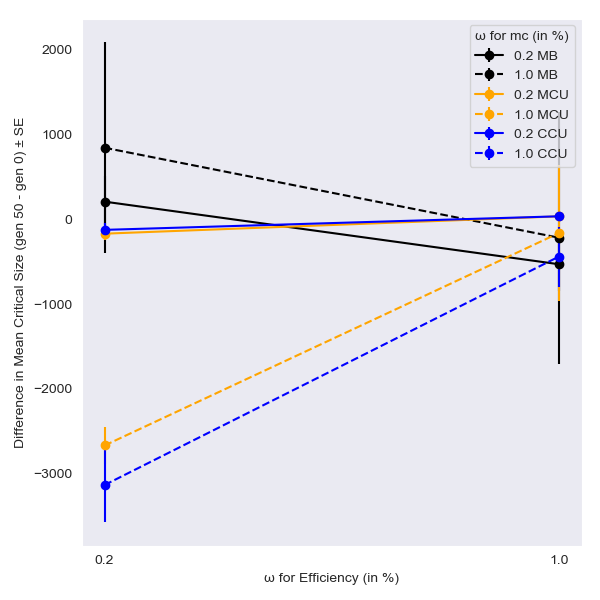
\includegraphics[width=0.5\textwidth]{C5/Figs/omg/omega_mc_eff_mc}
  }
  \subfloat{
  \centering
  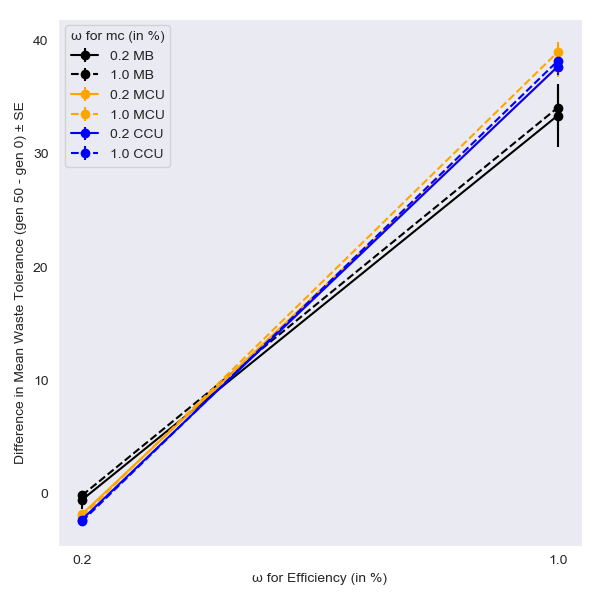
\includegraphics[width=0.5\textwidth]{C5/Figs/omg/omega_mc_eff_wtol}
  }
  \caption{Effect of heritability in critical size (mc) and efficiency on mean trait values at generation 50.}
  \label{fig:omg_mc_eff}
\end{figure}
\pagebreak
